\section{Problem analysis}
% \ninanotes{
% \begin{itemize}
% \item Coarse problem analysis Describing the problem and goals in more
% detail, briefly analysing the challenges, pointing out possible solutions.
% \item Problem specification and analysis Detailed specification of the
% problem (and goals). This might need to introduce new notation in order
% to arrive at a precise description. If relevant, make state-of-the-art
% solutions precise and compare.
% \item Goals and success criteria Describe the goals and when a goal is
% reached.
% \end{itemize}
% }

In this chapter I will go through the main difficulties in coming up with a good solution for Hanabi. Firstly I will go through hardware constraints, then I will motivate my overall solution using dynamic epistemic logic (DEL) and finally I will analyse some lower bounds on time and space this solution would lead to.

\subsection{Hardware and time constraints}
In order to run the self-play of the agents I will have to pick a platform to work on.
The setup I am gonna run the self-play of the agents on is utilizes an Intel® Core™ i7-10875H Processor, with 8 cores and 16 GB of ram. There are also 34GB of swap memory. So there is about 50 GB of memory as an constraint.
In regards to time constraint I want to make have that each agent does not spent much more time than a real-time player. A couple of minutes at most - but this goal is less important, but mostly there to secure that it is actually testable.
The chosen setup and time and memory constraints is mainly due to that is the computer I got, and I now I can iterate fast over a setup I have full control over.

\subsection{Multi-modal logic of \KTfourfiveN} \label{sec:definition-ktfourfiven}
In this problem I will have to use modal logic in order to solve the game of Hanabi. Modal logic is a field with a lot of depth and even notions like 'epistemic actions' can become part of the model\footnote{like \cite{EgerAndMartens17} logical system called Ostari}. I will chiefly focus on knowledge (what can be known) and what can be considered possible given the information an agent has. An approach to this is using \KTfourfiveN \cite{HuthAndRyan2004KT45n}, which seem flexible enough to adapt to the game. For completion, I put forward their definition of \KTfourfiveN in Figure \ref{fig:kt45n-definition}. 

To give a corrospondance to the Hanabi game, the world $w \in W$ will corrospond to some configuration of hands for all the players, and the deck, discard pile and color piles. Some equivalence relation $R_i = (w_x,w_y)$ means that player $i$ thinks that both $w_x$ and $w_y$ are possible based on the given information. And using the labelling function $L(w_k)$ could contain atoms like, "the first card in player $p$'s hand is able to be played" for world $w_k$, so it can be used to answer queries. 

Of course finding a good encoding for the worlds, such that it is easy to answer queries, as well as traversing the model in order to answer epistemic queries is no trivial task, and one might use a different encoding for a world than one strictly consisting of atoms (or booleans).





\begin{figure}
	\centering
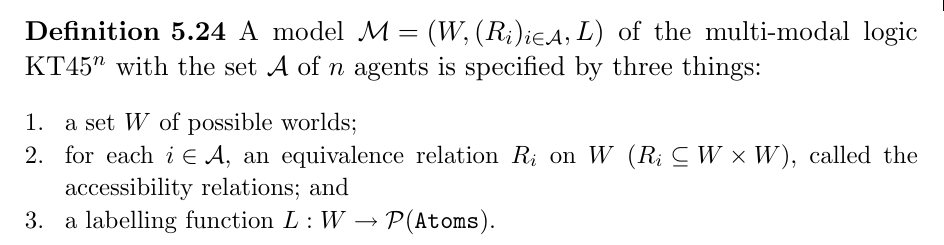
\includegraphics[width=13cm,frame]{images/kt45n-definition.png}
	\caption{Definition of \KTfourfiveN from \cite{HuthAndRyan2004KT45n}}
	\label{fig:kt45n-definition}
\end{figure}




\subsection{Problems with possible worlds and modal logic}
The problem with the approach of modal logic and possible worlds, is that we easily get combinatorial explosion. 
For some estimates on the number of possible hands for a single agent see Table \ref{table:combinations}.

\begin{table}
	\centering
\begin{tabular}{l|llll}
Number of players & 2       & 3       & 4       & 5      \\\hline
Min               & 65574   & 47666   & 7406    & 6676   \\
Max               & 93667   & 83848   & 16316   & 12962 
\end{tabular}
	\caption{The number of distinct combinations for an individual player as a function of the number of players in the game. On each column, I have data for 30 random games for $k$ players. In which I dealt the cards to all the players except for 1 player $p$, and calculated how many distinct combinations $p$ could get (see how data is generated by Appendix \ref{appendix:python-distinct-combinations}).}
	\label{table:combinations}
\end{table}


To give some lower bound on memory usage for the case of 2 players, we can take the minimum on the table 65574 and assume that we spent 1 bit on each possible generated world. This means that we would at least have 65574 for the POV player, and $65574^2$ for the other player (one for each fixed scenario). $65574^2$ alone is about 537GB which is completely infeasible given the hardware constraints. 
We do the same for calculating lower memory bound for 5 players, given that we generate a world for each fixed scenario, then we have at least $6676^2 \cdot 5$ worlds, which corrosponds to about 28GB, which is much more feasible given the constraints.
So the scenarios with 4 and 5 players seem to be the the least difficult to generate models for, or at least the models seem to be significantly smaller.
To optimize this approach, each agent could store the given hints and shown cards, and at some proper time -- when a significant amount of hints and cards have been revealed -- make the model of possible worlds. A different approach is to work with a smaller deck, which is what \cite{EgerAndMartens17} does, which has the added benefit ones ability to test the code in a fast manner, rather than waiting for lots of possible worlds to be generated and processed.

The main thing the program will spent its time on will be generating the possible worlds, and iterating through all possible worlds in order to answer some query. Just take the above analysis and replace "assume that we spent 1 bit on each possible generated world" with "assume that we spent 1 microsecond on each possible generated world", so I will have to find an efficient solution to generating $k$ distinct combinations from changing multisets, as well as efficient solution for iterating through it.

\subsection{Summary}
The main problems with trying to solve Hanabi is to both time and space constraints, where DEL, when applied naively, need to represent lot of possible worlds. 
I will have to use space-efficient data-structures in order to store the many possible worlds as well as fast algorithms for generating said possible worlds. 
Furthermore I will probably only be able to tackle the problem for 4 or 5 players, because otherwise there is not revealed enough information in order to substantially reduce the number of possible worlds.
